\documentclass[10pt,twocolumn,letterpaper]{article}

\usepackage{cvpr}
\usepackage{times}
\usepackage{epsfig}
\usepackage{graphicx}
\usepackage{amsmath}
\usepackage{amssymb}
% Include other packages here, before hyperref.
\usepackage[outdir=./]{epstopdf}

% If you comment hyperref and then uncomment it, you should delete
% egpaper.aux before re-running latex.  (Or just hit 'q' on the first latex
% run, let it finish, and you should be clear).
\usepackage[breaklinks=true,bookmarks=false]{hyperref}

% \cvprfinalcopy % *** Uncomment this line for the final submission

\def\cvprPaperID{****} % *** Enter the CVPR Paper ID here
\def\httilde{\mbox{\tt\raisebox{-.5ex}{\symbol{126}}}}

%% Custom control sequences
\let\oldPr\Pr
\newcommand{\bR}{\mathbb{R}}
\renewcommand*{\Pr}[1]{\mathbb{P}\left( #1 \right)}
\newcommand{\mat}[1]{\mathbf{#1}}
\DeclareMathOperator*{\argmax}{arg\,max}
\DeclareMathOperator*{\argmin}{arg\,min}
\newcommand{\tr}{\mathbf{tr}}
\newcommand{\cross}[1]{[#1]_{\times}}


% Pages are numbered in submission mode, and unnumbered in camera-ready
%\ifcvprfinal\pagestyle{empty}\fi
\setcounter{page}{4321}
\begin{document}

%%%%%%%%% TITLE
% \title{All Graphs Lead to Rome: \\
% Cycle Consistent Multi-View Representations Using Graph CNNs}
\title{All Graphs Lead to Rome: Learning Geometric and Cycle Consistent Representations with Graph CNNs}

\author{Stephen Phillips, Kostas Daniilidis \\
GRASP Labratory, University of Pennsylvania\\
{\tt\small \{stephi, kostas\}@seas.upenn.edu}
% For a paper whose authors are all at the same institution,
% omit the following lines up until the closing ``}''.
% Additional authors and addresses can be added with ``\and'',
% just like the second author.
% To save space, use either the email address or home page, not both
% \and
% Second Author\\
% Institution2\\
% First line of institution2 address\\
% {\tt\small secondauthor@i2.org}
}

% When placing figures in \LaTeX, it's almost always best to use
% \verb+\includegraphics+, and to specify the  figure width as a multiple of
% the line width as in the example below
% {\small\begin{verbatim}
%    \usepackage[dvips]{graphicx} ...
%    \includegraphics[width=0.8\linewidth]
%                    {myfile.eps}
% \end{verbatim}
% }


\maketitle
%\thispagestyle{empty}

% Papers, excluding the references section,
% must be no longer than eight pages in length. The references section

%%%%%%%%% ABSTRACT
\begin{abstract}
   % Put abstract here
   % OK I hate this start but we will work on it.
   (Work in progress) In this work we present a learning technique for refining multi-image matches in an unsupervised fashion.
   We formulate the multi-image matching problem as a graph embedding problem then use recent work in Graph Neural Networks to learn the appropriate embedding function.
   Since ground truth correspondence is difficult or expensive to come by in many real world datasets, we use cycle consistency as our loss function.
   Additional losses can be added if more information is available in the training set for better test performance.
   To the best of our knowledge, no other works have used learning for multi-image feature matching.
   Our experiments show that our method is competitive with other optimization based approaches.
\end{abstract}

%%%%%%%%% BODY TEXT
\section{Introduction}

% TODO: Add more citations
Feature matching is an essential part of many geometric computer vision applications.
Much work has been done on image matching for the last several decades \cite{fischler1981random}.
However we still have not fully answered the question: What are the best image features to describe multiple views of the same scene?
Recently deep learning has revolutionized how image features are computed \cite{yi2016lift}, and we would like to leverage this to compute better scene features.
Typically when applied to this area, deep neural networks (DNNs) are trained with photometric losses.
Photometric losses make the brightness constancy assumption, which is not as robust as feature matching.
Can we learn using multi-view constraints directly?

\begin{figure}[t]
\begin{center}
  % \fbox{\rule{0pt}{2in} \rule{0.9\linewidth}{0pt}}
  \includegraphics[width=0.8\linewidth]{figures/CycleConsistencyBasic.pdf}
\end{center}
  \caption{
    Example of multi-image matching, with images from Rome16K dataset \cite{li2010location}.
    Shown is an example of an error in matching leading to an inconsistency cycle.
    In this work, we show how to learn this multi-view matching problem.
  }
\label{fig:cycconsistex}
\label{fig:onecol}
\end{figure}


Unfortunately, there are obstacles to applying multi-view constraints directly to learning. 
To train networks, we need a large amount of labelled data.
In the case of multi-image feature matching, one would need to hand label point correspondences between images, which is difficult and expensive to obtain.
Multi-view constraints are formulated in terms of sparse features, thus traditional convolutional deep neural nets (CNNs) are not designed to handle such input.
In the case of multi-image feature matching, geometric constraints would be helpful in rejecting outlier matches.

In this work, we propose to solve these problems using a Graph Neural Network (GNN) to operate on the correspondence graph.
The method proposed works on the correspondence graph, agnostic to how correspondnces were computed.

We use a self-supervised loss, the cycle consistency loss, to train the network.
We also add in side geometric losses to help training, which works even when the geometric information is not available at test time.
Our contributions are:
\begin{itemize}
\item A novel architecture for multi-image feature matching using GNNs with graph embeddings
\item The use of the self-supervised cycle consistency loss
\item Test geometric consistency losses toward the training
\item Perform experiments on the Rome16K \cite{li2010location} dataset to test the effectiveness of our method compared to the optimization based baselines
\end{itemize}


%-------------------------------------------------------------------------
\section{Related Work}

Matching has a rich history of research in computer vision.
The most well known and widely used method for image matching is that of RANSAC \cite{fischler1981random}.
RANSAC combined with hand-crafted feature descriptors like SIFT \cite{lowe2004distinctive}, SURF \cite{bay2006surf}, BRIEF \cite{calonder2012brief}, or ORB \cite{mur2015orb} has constituted the bulk of the matching literature for the last 40 years.
To improve matching of all the features of the image, graph matching \cite{suh2015subgraph, hu2016distributable} can also be used for more robust matching.

Multi-image matching has traditionally been done using optimization based methods minimizing a cycle consistency based loss (see Section 3.3) such as \cite{pachauri2013solving,zhou2015multi,arrigoni2017synchronization} and \cite{wang2017multi}.
\cite{pachauri2013solving} and \cite{arrigoni2017synchronization} use the eigenvectors of the matching matrix to obtain a low dimensional embedding. 
Thus they are robust to small Gaussian noise but not to stronger noise.
\cite{zhou2015multi} and \cite{wang2017multi} use most sophisticated optimization techniques on the matching matrix and thus are quite robust.
However, they use a centralized scheme and thus are not appropriate in a distributed setting,
as done in \cite{leonardos2016distributed}.
There are also density based optimization techniques to compute multi-image correspondence, such as in \cite{tron2017fast}.

Previous attempts to improve image matching techniques using machine learning have focused on learning the descriptors given ground truth correspondence from curated datasets \cite{zagoruyko2015learning, yi2016lift, brachmann2017dsac}. This approach is limited if you do not have the ability to get the ground truth correspondences.
There are other methods to build correspondences \cite{choy2016universal}, but it only handles two-view constraints and requires dense correspondences.
Most similar to ours, \cite{yi2018learning} attempts to improve correspondences by learning match probabilites for RANSAC to speed up test time running. However, they only focus on two view tests and do not exploit the advantages of the correspondence structure.

Graph neural networks have been getting more attention recently 
\cite{bronstein2017geometric, bruna2013spectral, defferrard2016convolutional, kipf2016semi, scarselli2009graph, gama2018mimo, gama2018convolutional, battaglia2018relational}.
Classical so-called Spectral methods used the eigenvectors of graph Laplacian to compute convolutions \cite{bronstein2017geometric}, but this requires a fixed graph structure known a-priori.  
Non-spectral methods do not have this requirement \cite{bronstein2017geometric, kipf2016semi, scarselli2009graph, gama2018convolutional}. Most of these simply use polynomials of the graph Laplacian to compute neighborhood averages. \cite{gama2018mimo} and \cite{gama2018convolutional} formalize this notion and generalize it beyond the use of the graph Laplacian. More sophisticated aggregation techniques and global information passing can also be used as discussed in \cite{battaglia2018relational}.

%------------------------------------------------------------------------
\begin{figure*}[t]
\begin{center}
  % \fbox{\rule{0pt}{2in} \rule{0.9\linewidth}{0pt}}
  \includegraphics[width=0.8\linewidth]{figures/CycleConsistencyMainFigure.pdf}
\end{center}
  \caption{
    An outline of the pipeline of this work.
    The graph of matches is put to a Graph Convolutional Neural Network (GCN) \cite{kipf2016semi} then creates a low rank embedding of the Adjacency Matrix of the graph.
    The GCN operates on an embedding over the nodes the graph.
    The colors on the nodes of the graph in the GCN represent the values of the embedding.
    The final embedding is used to construct a pairwise similarity matrix, which ideally should be a low dimensional representation of the graph adjacency matrix i.e. should be a cycle consistent version of the graph adjacency matrix.
    We train the network using a reconstruction loss on the similarity matrix.
    In addition we can use geometric information at to assist training the network, even if we do not have that geometric information at testing time.
    This can be epipolar constraints on the point locations or higher order geometric constraints.
  }
\label{fig:pipeline}
\label{fig:onecol}
\end{figure*}

\section{Method}
Our goal is to learn optimal features that capture multiple image views.
We formulate this problem in terms of the correspondence graph of the features.
We denote vectors $\mat{x}$ and matrices $\mat{A}$ with boldface.
We denote the $i^{th}$ row of a matrix $(\mat{A})_i$.
\subsection{Correspondence Graph}
We assume we have an initial set of feature matches represented as a graph $\mathcal{G} = (\mathcal{V}, \mathcal{E})$.
Each vertex $v$ of the graph is a feature with its associated descriptor $f_v$. 
The graph is represented by its Weighted Adjacency Matrix $\mat{A}(\mathcal{G}) \in \bR^{n \times n}$ and its positive diagonal degree matrix $\mat{D}(\mathcal{G}) \in \bR^{n \times n}$ (denoted $\mat{A}$ and $\mat{D}$ for brevity).
We can get an embedding matrix $E_0$ by combining the features $f_v$ from each of the vertices.
We use $E_0$ as our initializiation for our learning algorithm.
We can also add any additional knowledge we have into the embedding (e.g. scale, orientation, etc.).
Putative correspondences are computed from these features and represented by weighted edges in which the weight gives the strength of the match.
While there are many interesting methods for computing these putative correspondences \cite{suh2015subgraph, yi2018learning}, we do not explore them in this work.

In the absence of noise or outliers, this graph would have $p$ disjoint connected components, where $p$ is the number of co-visible points in the world.
Each feature would only have edges to other features corresponding to the same point.
Since features in this case represent unique location in the scene, no points in the same image would have edges between them.
Typically putative correspondences match probabilistically, meaning a feature in one image matches to many features in another.
This could come from repeated structures in the scene, ambiguity from the low-level feature descriptors, or just an error in the matching algorithm.
Filtering out these noisy matches is our primary learning goal.

However, this graph structure does not have the properties of a Eulcidean domain.
Thus we cannot use standard CNNs to learn features for this task.
Thus we need to use graph convolutions to learn feature representations on this space, which we explore in this next section.

\subsection{Graph Neural Networks}
Much attention has been given to graph neural networks (GNNs) recently
\cite{bronstein2017geometric, bruna2013spectral, defferrard2016convolutional, kipf2016semi, scarselli2009graph, gama2018mimo, gama2018convolutional, battaglia2018relational}.
Modern GNNs use non-spectral methods, such as the following:
\begin{align}
      \mat{L} =&\; I - \mat{D}^{-1/2} \mat{A} \mat{D}^{-1/2} \\
\mat{E}_{i+1} =&\; P\left(\sigma\left( \sum_k \mat{L}^k \mat{E}_i \mat{W}_{i,k} \right)\right)
\end{align}
The matrix $L$ is the graph Laplacian, use to encode the graph structure, and $\mat{W}_{k,i}$ are the learned weights of layer $i$.
The degree of the polynomial determines the number of hops away from a node one layer can access.
Here $\sigma$ is the non-linearity (typically a ReLU) and $P$ is the `pooling' operation, known as graph coarsening \cite{bronstein2017geometric, gama2018mimo}.
As we need an embedding over the whole graph, we cannot perform graph coarsening, and thus we only perform the non-linearity step.

We instead use a modification of the approach in \cite{kipf2016semi}:
\begin{align}
      \widetilde{\mat{L}} =&\; (\mat{D} + \mat{I})^{-1/2} (\mat{A} + \mat{I}) (\mat{D} + \mat{I})^{-1/2} \\
\mat{E}_{l+1} =&\; \sigma\left(\widetilde{\mat{L}} \mat{E}_i \mat{W}_i \right)  \label{eq:graph_conv}
\end{align}

The matrix $\widetilde{L}$ is analogous to the graph Laplacian (with better numerical stability properties).
$\widetilde{L}$ is used to encode the structure of the graph and is used to perform the actual graph convolution.
We use many layers, and thus the receptive field of the final embedding is quite large, even without the pooling operations.
For simplicity we restrict ourselves to this for now, though in principle we could use higher hop neighborhoods \cite{gama2018convolutional}, or more complicated aggregation structures \cite{battaglia2018relational}.
The final output $\mat{E}_n$ gives us a new descriptor for every node.
In the next sections we will discuss the loss functions to train this network.

\subsection{Cycle Consistency}
If the pairwise matches are globally consistent, then we can say that, for all $i, j, k$:
\begin{equation}
\mat{M}_{ij} = \mat{M}_{ik} \mat{M}_{kj}
\label{eq:cycconsist1}
\end{equation}
In other words, the matches between two images stays the same no matter what path is taken to get there. 
This constraint is known as \textit{cycle concistency}, and has been used in a number of recent works to optimize for global consistency \cite{zhou2015multi, wang2017multi, leonardos2016distributed}.
Stated in this form, there are $O(n^3)$ cycle consistency constraints to check.
A more elegant way to represent cycle consistency is to first create a `universe' of features that all images match to.
Then one can match the $i^{th}$ set of features to the universe, denoted $\mat{X}_i$.
Then the cycle consistency becomes:
\begin{equation}
\mat{M}_{ij} = \mat{X}_{i}\mat{X}_{j}^\top
\label{eq:cycconsist2}
\end{equation}

% In our case, we try to learn embeddings $\mat{E}$ that map to the $\mat{X}_i$ - learn the universe of features via our embeddings.
We try to learn $\mat{E}$ to approximate $\mat{X}$ - in other words the final embedding should be an encoding of the universe of features.
Thus our loss would be 
\begin{equation}
\mathcal{L}(\mat{A}, \mat{E}_n) = \mathcal{D}(\mat{A}, \mat{E}_n\mat{E}_n^\top)
\end{equation}
Here $\mathcal{D}$ could be an $L_2$ loss, $L_1$ loss, or many others. 
Another way of viewing this is that features $i$ and $j$ match with probability $(\mat{E}_n)_i \cdot (\mat{E}_n)_j$ which is proporitional to $\mat{A}_{ij}$.

\begin{figure}[t]
\begin{center}
  \includegraphics[width=0.8\linewidth]{figures/GeometricConsistency.pdf}
\end{center}
  \caption{
    Illustration of the Geometric loss.
    We compute the errors on each feature match to determine their validity.
    Errors are computed via absolute distance from the epipolar line, as expressed by equation \ref{eq:essential_constraint} via the epipolar constraint.
  }
\label{fig:cycconsistex}
\label{fig:onecol}
\end{figure}

\subsection{Geometric Side Information}
One of the main advantages of this approach over more traditional optimization based approaches is the ability to add geometric side information into the loss at training time, even if it is not available at test time.
The simplest way to add this, and the approach we use here, is using the epipolar constraint.
The epipolar constraint describes how the positions of features in different images corresponding to the same point should be related.
Given a relative pose $(R_{ij}, T_{ij})$ between two cameras $i$ and $j$  (transforms $j$ to $i$) the epipolar on corresponding feature locations $X_i$ and $X_j$:
\begin{equation}
X_{i}^\top \cross{T_{ij}}R_{ij} X_{j} = 0
\label{eq:essential_constraint_rel}
\end{equation}
In this work we use the two pose epipolar constraint \cite{tron2014quotient}:
\begin{equation}
X_{i}^\top R_{i}^\top \cross{T_{j} - T_{i}}R_{j} X_{j} = 0
\label{eq:essential_constraint}
\end{equation}
% Where the $(R_k, T_k)$ are the poses of cameras $i$ and $j$ respectively.
This assumes that the $X_k$ are calibrated i.e. the camera intrinsics are known. 
Given the matrix of correspondences between camera $i$ and $j$, $\mat{M}_{ij}$, we can formulate this as a loss:
\begin{equation}
\mathcal{L}_{ij,geom}(\mat{M}_{ij}) = \sum_{k,l} (\mat{M}_{ij})_{kl} \left|X_{i,k}^\top R_{i}^\top \cross{T_{j} - T_{i}}R_{j} X_{j,l}\right|
\label{eq:geom_cost}
\end{equation}
For our purposes, since we use low rank embeddings of the $\mat{M}_{ij}$, the loss would look like:
\begin{align}
\mathcal{L}_{geom}(\mat{E})
=&\; \mathrm{tr}(\mat{G}^\top \mat{E}\mat{E}^\top) = \sum_{i,j} (\mat{E})_{i} \cdot (\mat{E})_{j} (\mat{G})_{ij} \\
(\mat{G})_{ij} =&\; \left|X_{i}^\top R_{c(i)}^\top \cross{T_{c(j)} - T_{c(i)}}R_{c(j)} X_{j}\right| \nonumber
\label{eq:geom_cost2}
\end{align}
Where $c(i)$ is the appropriate camera for point index $i$.
While this is all we use in this work, in principle you could use higher order constraints such as the trifocal tensor as additional loss terms.


%------------------------------------------------------------------------
\section{Experiments}

\begin{figure*}
\begin{center}
  % \fbox{\rule{0pt}{2in} \rule{.9\linewidth}{0pt}}
  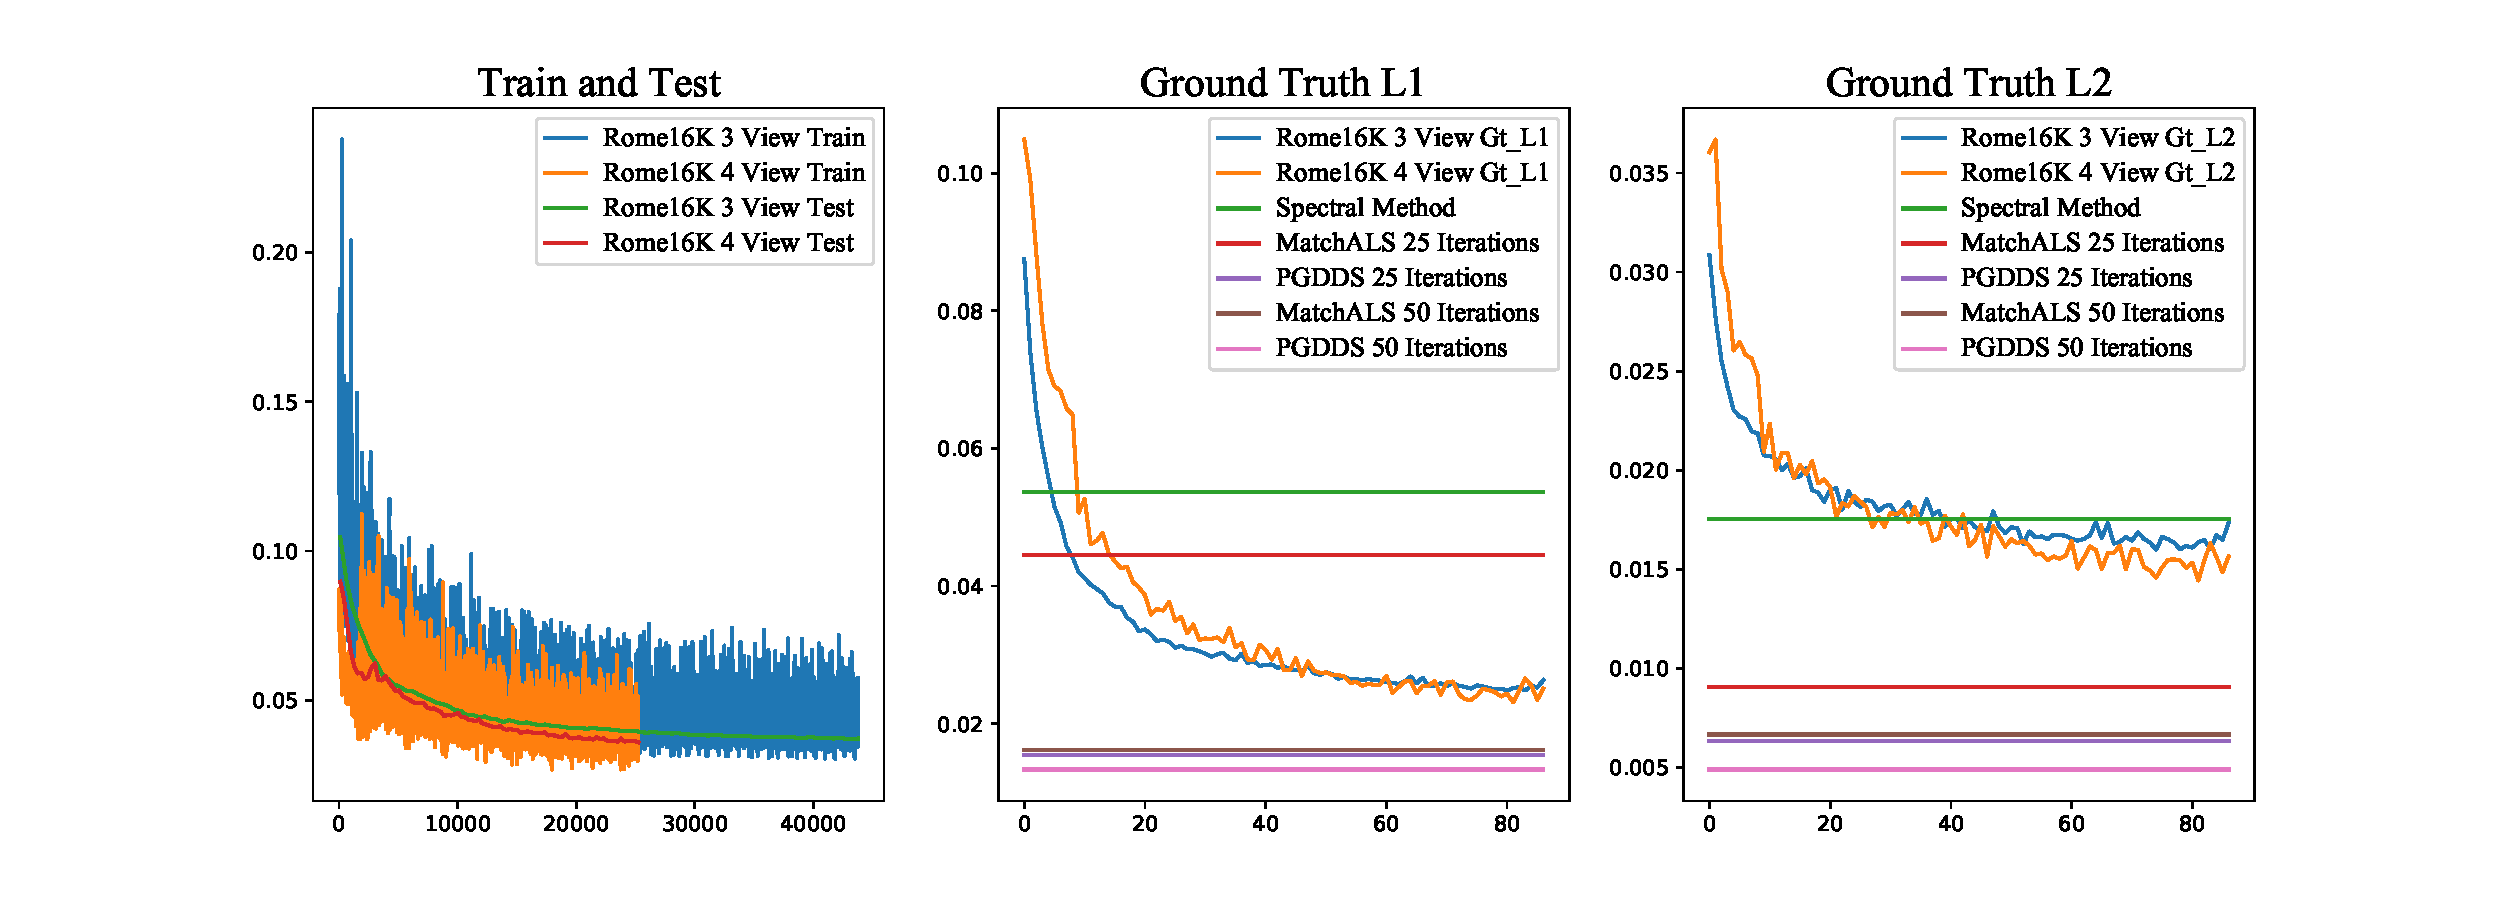
\includegraphics[width=0.8\linewidth]{figures/TrainingCurves.pdf}
  \end{center}
    \caption{
      Training curves with and without Geometric Training loss.
      The training loss dramatically improves training time and performance.
      Shown as horizontal lines are the state of the art optimization based baselines.
      Even with a simple network we compare well with them.
      NOTE TO READERS: This figure needs to be cleaned up.
    }
  \label{fig:short}
\end{figure*}

\begin{figure*}
\begin{center}
  % \fbox{\rule{0pt}{2in} \rule{.9\linewidth}{0pt}}
  \includegraphics[width=0.8\linewidth]{figures/experiments01-eps-converted-to.pdf}
  \end{center}
     \caption{Experimental results from Rome16K}
  \label{fig:short}
\end{figure*}

\begin{table*}
\begin{center}
\begin{tabular}{|l|c|c|}
\hline
Method & Same Point Similarities & Different Point Similarities  \\
\hline\hline\hline
Ideal                              & 1.00e+0 $\pm$ 0.00e+0 & 0.00e+0 $\pm$ 0.00e+0 \\ \hline
Initialization Baseline            & 5.11e-1 $\pm$ 1.68e-2 & 2.56e-1 $\pm$ 2.06e-1 \\ \hline
3 Views, Noiseless                 & 9.96e-1 $\pm$ 7.70e-3 & 1.16e-1 $\pm$ 1.32e-1 \\ \hline
5 Views, Noiseless                 & 1.00e+0 $\pm$ 4.15e-4 & 1.22e-1 $\pm$ 1.67e-1 \\ \hline
3 Views, Added Noise               & 9.96e-1 $\pm$ 7.70e-3 & 1.16e-1 $\pm$ 1.32e-1 \\ \hline
3 Views, Added Noise               & 9.68e-1 $\pm$ 5.29e-2 & 9.50e-2 $\pm$ 1.58e-1 \\ \hline
5 Views, Added Noise               & 9.89e-1 $\pm$ 2.47e-2 & 7.67e-2 $\pm$ 1.56e-1 \\ \hline
6 Views, Added Noise               & 9.84e-1 $\pm$ 3.16e-2 & 7.46e-2 $\pm$ 1.57e-1 \\ \hline
3 Views, 5\% Outliers              & 9.29e-1 $\pm$ 1.79e-1 & 1.41e-1 $\pm$ 1.48e-1 \\ \hline
3 Views, 10\% Outliers             & 9.27e-1 $\pm$ 1.79e-1 & 1.40e-1 $\pm$ 1.51e-1 \\ \hline

\hline
\end{tabular}
\end{center}
\caption{
Results on Rome16k Correspondence graphs.
Losses tested against ground truth correspondence graph adjacency matrices.
Our method was not trained on ground truth corresopndences but on unsupervised methods.
}
\end{table*}
\subsection{Synthetic Graph Dataset}
We test our method on synthetically generated data as a simple proof of concept.
To generate the data, we generate $p$ points, each with its own randomly generated descriptor.
To create the graph, we generate random permutation matrices, with a noise applied to it after it is generated.
The initial descriptors we created using the true descriptor plus some added noise.
No geometric losses were added during training for these experiments.
Testing with different noise functions and parameters.
All experiments were run with a 12 layer GCN with the ReLU nonlinearity and skip connections between the first layer and the 6th and 12th layers.
All were trained with the Adam optimizer and a learning rate $10^{-4}$


\subsection{Rome 16K Graph Dataset}
% Filler for now.
% TODO: Actually run tests on all these with different loss functions
We  use the Rome16K dataset \cite{li2010location} to test our algorithm in real world settings.
We extract image triplets, quadtruplets, and quintuplets with overlap of 80 points or more to test our algorithm on. For the normal datasets, we extracted 80 points established as corresponding in the bundle adjument given in the Rome16K dataset. For the outlier datasets, we take 79 correspondences and 1 non-corresponding point in each image.

We test with various loss functions, specifcally $L_1$, $L_2$, and the binary cross entropy loss (BCE).
We evaluate on a test set using the ground truth Adjacency matrix which we compute from the bundle adjustment given by the Rome16K dataset.
Traditional methods of evaluation use Precision and Recall, after making the labels 0 or 1.
We forgo this as our method was trained to output soft labels - we also in turn make the labels soft for the optimization based methods.
We also include ablation studies on various geometric loss functions for the geometric side information.

% leaderConsensus.m  MatchALSTestErrors.txt  mmatch_CVX_ALS.m  mmatch_QP_PG.m  mmatch_spectral.m  PGDDS.m  PGDDSTestErrors.txt  print_errors.py  run_tests.m  SpectralTestErrors.txt

\begin{table*}
\begin{center}
\begin{tabular}{|l|c|c|c|}
\hline
Method & L1 Loss & L2 Loss & BCE Loss \\
\hline\hline\hline
Spectral                                  & 5.368e-2 $\pm$ 5.274e-3 & 1.754e-2 $\pm$ 3.688e-3 & 1.143e-1 $\pm$ 2.774e-2 \\ \hline
MatchALS                                  & 6.715e-3 $\pm$ 3.035e-3 & 6.696e-3 $\pm$ 3.035e-3 & 2.254e-1 $\pm$ 1.043e-1 \\ \hline
PGDDS                                     & 1.311e-2 $\pm$ 2.186e-3 & 4.730e-3 $\pm$ 1.886e-3 & 3.872e-2 $\pm$ 3.869e-2 \\ \hline
GNN, 12 Layers, w/o Geometric Side Losses & 1.000e-3 & 1.000e-3 & 1.000e-3 \\ \hline
GNN, 12 Layers, w/ Geometric Side Losses  & 1.000e-3 & 1.000e-3 & 1.000e-3 \\ \hline
\hline
\end{tabular}
\end{center}
\caption{
Results on Rome16k Correspondence graphs.
Losses tested against ground truth correspondence graph adjacency matrices.
Our method was not trained on ground truth corresopndences but on unsupervised methods.
}
\end{table*}





%------------------------------------------------------------------------
\section{Conclusion}

We have shown a novel method for training feature matching.
We have demonstrated its effectiveness using experiments on the Rome16K dataset.
This method can be employed even when labelled training data is not available, but can still incorporate side geometric information.
For future work we hope to use more robust losses for outlier rejection, and to incorporate learning image level features into this pipeline.

{\small
\bibliographystyle{ieee}
\bibliography{mybib}
}

\end{document}
